\chapter{SourceMeter szoftvercsalád}
\label{chap:fejezet2}

A SourceMeter eszközkészlet statikus forráskód elemző szoftvercsomag, mely különböző nyelvek elemzéséhez tartalmaz elemző és detektáló szoftvereket. Ezen eszközök segítségével a támogatott nyelvekben írt projektekben többek között gyengepontokat és kódolási szabálysértéseket mutat ki egy egységes, nyelvfüggetlen módon.
A SourceMeter statikusan elemzi a bemenetként kapott projekteket. 

Statikus elemzés során a vizsgált kódbázis futtatás nélkül van vizsgálva szintaktikai és szemantikai szempontból. A szintaxis elemzés az alkalmazás forráskódjának felépítését és szintaxisát vizsgálja, hogy érvényes-e a programozási nyelv szabályai szerint. A szemantikus elemzés azonban a kód mögötti logikát vizsgálja, hogy az megfelel-e az adott feladatnak és az elvárásoknak. 

Az eszközkészlet többek között a C, C++, Java, RPG, és a JavaScript nyelvekben írt projektek kódbázisának mély elemzését támogatja 
Kódbázis elemzés elvégzéséhez előre összeállított sémák alapján a bemenetként kapott projekt elemeiből többek között Absztrakt Szintaxis Fát (AST) állít elő, melynek feldolgozása során különböző metrikákat számol ki, például logikai kódsorok száma (LLOC, avagy Logical Lines Of Code), kód beágyazások mélysége (NL, avagyNesting Level), vagy megjegyzések sűrűsége (CD, avagy Comment Density). Ezek mellett kódolási szabálysértések és duplikált kódsorok detektálására is alkalmas az eszközkészlet adott szoftverjei.

A SourceMetert eszközkészletet egy másik forráskód elemző eszközben, a Sonar Qube-on belül is használhatjuk bővítményként. A SourceMeter és a SonarQube közötti integráció lehetővé teszi a fejlesztők számára, hogy a SourceMeter eredményeit a SonarQube-ba exportálják, melynek köszönhetően könnyen összehasonlíthatóak az elemzési eredmények. Az integráció lehetővé teszi a fejlesztők számára, hogy a SonarQube felületén keresztül megjelenítse és kezelje a SourceMeter eredményeit, és hogy integrálják az elemző eszközöket a fejlesztési folyamatukba.

A SonarQube-on kívül a QualityGate nevű szoftver is felhasználja a SourceMeter szoftvercsomagjait. A QualityGate a SourceMeter által készített metrikákat és jelentéseket használja az alkalmazás minőségének és biztonságának értékeléséhez, és automatikusan jelzi a fejlesztőknek, ha az alkalmazás nem felel meg a meghatározott küszöbértékeknek. Ez segíti a fejlesztőket abban, hogy gyorsan és hatékonyan javítsák az alkalmazásukat, és biztosítják, hogy az megfelelő minőségű és biztonságos legyen.

Mindegyik szoftvercsomaghoz tartozik az elemzett nyelv alapján egy előre elkészített séma, mely egy Absztrakt Szemantikus Gráfot, másnéven ASG-t tartalmaz. Az elemzés lépései során ezek alapján végzik feladataikat a csomag programjai. Ezek lehetnek Absztrakt Szintaxis Fa, avagy AST felépítése, metrikák számolása, kódolási szabálysértések keresésére és ezek mindegyikének felhasználása duplikált kódszegmensek detektálására.
Ezen sémák az elemzett nyelvnek nyelvtanának és szemantikájának megfelelő szerkezetét tartalmazzák, melyekben a csomópontok adott nyelvtani elemeket, az élek pedig az elemek közötti kapcsolatot reprezentálják. Egy példa erre \aref{fig:sema_pelda} ábrán látható:

\begin{figure}[!htbp]
    \caption{Sémában található elemek, kapcsolataik}\label{fig:sema_pelda}
    \centering
    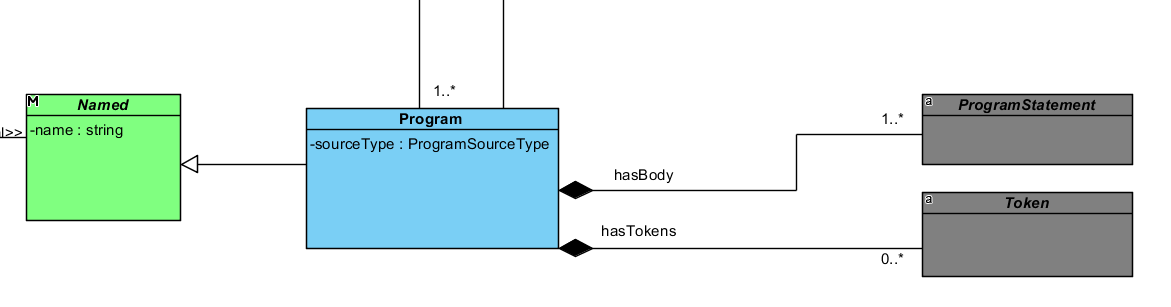
\includegraphics[width=0.9\textwidth]{sema_pelda.png}
\end{figure}

A SourceMeter szoftvercsomagjai a mély elemzés különböző lépéseit több program használatával végzi el, melyek a folyamat során speciális feladatokat látnak el. A SourceMeter for JavaScript esetén az elemzés fő lépéseit 14 program végzi el, melyek mellett a szoftvercsomag előkészítéséhez fordítás során egyéb segédprogramok is fel vannak használva. Ezek közül szakdolgozatom feladata során az alább említett programokban lesznek bővítések és módosítások megvalósítva.

Az elemzés első lépésében a JSAN futtatásával az elemzendő projekt kódbázisából egy egyedi absztrakt szintaxisfát készít, mely többek között tartalmazza a projekt nyelvtani struktúráját és egyéb, függvényhívásokhoz tartozó információkat. Ezt későbbi lépések során metrikák számolására és duplikált kódszegmensek detektálására lehet felhasználni.

Az ESLintRunner program futtatásával a bemeneti kódbázisban különböző kódolási szabálysértéseket keres, melyek pontos helyét egy \texttt{.xml} formátumú fájlban összegzi. A detektált szabálysértéseket különálló szabályfájlok (későbbiekben \texttt{.rul.md} fájlok) használatával lehet megadni, melyek Markdown jelölőnyelven vannak megírva. Ezen fájl hiányában a program egy alapértelmezett, \texttt{.json} formátumban megadott szabályfájl használatával fogja az elemzést végrehajtani.

A JavaScript CallGraph (továbbiakban JSCG) az elemzett kódbázis alapján egy hívásgráfot (\texttt{callgraph}) állít elő. A hívásgráf (amelyet hívásmultigráfnak is neveznek) egy irányítási folyam-gráf, amely megjeleníti a részprogramok közötti hívási kapcsolatokat egy számítógépes programban. Minden csomópont egy eljárást képvisel, és minden él (f, g) jelzi, hogy az f eljárás hívja a g eljárást. Ez a gráf a JSAN által generált kimenetbe van beágyazva.

A SchemaGenerator egy segédprogram, mely a szoftvercsalád fordítása során az előre meghatározott sémákból előállított ASG fájlok alapján generál futtatáshoz szükséges állományokat. A SourceMeter for JavaScript fordítása esetében a JSAN futtatásához szükséges \texttt{javascriptAddon.node} fájl generálását végzi, mely segítségével az elemzett nyelvtani elemeket beágyazza 'burkoló csomagpontba', másnéven 'wrapper'-ekbe. A nyelvtani elemeket és a hozzájuk tartozó információkat a szoftvercsalád programjai ezeknek a wrappereknek segítségével tudják elérni és felhasználni. Ez a feladat során kibővül további fájlok generálásához szükséges funkciókkal.

